\documentclass[xcolor=dvipsnames]{beamer}
%
\usetheme{ESSLLI}
\setbeamercovered{transparent}

\usepackage{listings}

\usepackage{amsmath,amsfonts}
%\usepackage{stmaryrd}
%\usepackage{beamerthemesplit}
\usepackage{qtree}
\usepackage{tipa}

\allowdisplaybreaks[1]

\parindent0mm
\parskip7pt

\usepackage{textpos}
\usepackage{setspace}
\usepackage{color,colortbl}

\newcommand{\code}[1]{\colorbox{black!80}{\parbox{11cm}{\color{LightGrey}\tt #1}}}
\definecolor{CWIred}{HTML}{C41230}

\usepackage{tikz}
\usetikzlibrary{arrows,chains,matrix,positioning,scopes,shadows,backgrounds,fit,calc}

\def\firstcircle{(0,0) circle (1.5cm)}
\def\secondcircle{(0:1cm) circle (.05cm)}
\def\thirdcircle{(0:2cm) circle (1.5cm)}


\usepackage{phaistos}
\usepackage{stmaryrd,verbatim}

\newcommand{\sem}[1]{\ensuremath{[\hspace{-1.8pt}[ #1 ]\hspace{-1.8pt}]}}
\newcommand{\semmg}[1]{\ensuremath{[\hspace{-1.8pt}[ #1 ]\hspace{-1.8pt}]^{M,g}}}
\newcommand{\textsem}[1]{\ensuremath{[\hspace{-1.8pt}[ \text{#1} ]\hspace{-1.8pt}]}}


\title[Computational Semantics]{Computational Semantics\\ Day 3: Lambda calculus\\ and the composition of meanings}
%\author[Jan van Eijck \& Christina Unger]{Jan van Eijck$^1$ \& Christina Unger$^2$}
%\institute[]{$^1$CWI, Amsterdam, and UiL-OTS, Utrecht, The Netherlands\\ $^2$CITEC, Bielefeld University, Germany}
%\date[ESSLLI 2011]{ESSLLI 2011, Ljubljana}

%%%%%%%%%%%%%%%%%%%%%%%%%%%%%%%%%%%%%%%%%%%%%%%%%%%%%%%%%%%%%%%%%%%%%%%%%%%%%

\begin{document}

\lstset{language=Haskell,basicstyle=\footnotesize\ttfamily,frame=single,showstringspaces=false}

%\setbeamertemplate{footline}[split]
\setbeamercovered{invisible}

\begin{frame}{\ \ }
\titlepage
\end{frame}

%%%%%%%%%%%%%%%%%%%%%%%%%%%%%%%%%%%%%%%%%%%%%%%%%%%%%%%%%%%%%%%%%%%%%%%%%%%%%

\section{Lambda calculus}


\section*{Outline}
\begin{frame}{Outline}
\tableofcontents
\end{frame}


\begin{frame}{\ \ }

\begin{center}
{\Large Lambda calculus}

\vspace{1cm}

{\footnotesize
\parbox{6cm}{{\em\large Lambdas changed my life.}\begin{flushright}(Barbara H. Partee)\end{flushright} }

\parbox{6cm}{{\em\large All you need is lambda.}\begin{flushright}(Simon Peyton-Jones)\end{flushright} }
}
\end{center}
\end{frame}

\subsection{A short history}

\begin{frame}{}

\begin{center}
{\Large A short history}
\end{center}
\end{frame}

\begin{frame}{History}

\parbox{8cm}{{\bf Leibniz' ideal:}
\begin{itemize}
\item Create a universal language in which all possible problems can be stated. 
\item Find  a decision method to solve all problems stated in this universal language.
\end{itemize}} 
\parbox{2.5cm}{\includegraphics[width=2.5cm]{bilder/leibniz1.jpg}}

Considering only mathematical problems, set theory (formulated in the language of  
first order predicate logic) can serve as the universal language. 

However, it is not possible to solve all problems formulated in that language. 
To prove this, a formalization of the intuitive notion of {\em decidability} 
(or: {\em computability}) was necessary. 
\end{frame}

\begin{frame}{History}

In 1936, Turing and Church independently introduced two equivalent models of computation: \\ 
\parbox{7cm}{
\begin{itemize} 
\item {\bf Alan Turing: Turing Machine}\\ 
{\small A function is computable if a sequence of instructions can be specified and then carried out by 
a simple abstract computational device.}\\[2ex]
\item {\bf Alonzo Church: Lambda Calculus}\\ 
{\small Every computable function is a function that is definable in the lambda calculus.}
\end{itemize}}
\parbox{1cm}{\ }
\parbox{2cm}{
\includegraphics[height=2.5cm]{bilder/alanturing.jpg}\\[1ex] \includegraphics[height=2.5cm]{bilder/church.jpg}}\\[1ex]
Both models proved to be equivalent, i.e. capture the same class of functions.
\end{frame}

\begin{frame}{Connection to programming languages}

\begin{itemize}
\item {\bf Imperative programming languages} are based on the way a Turing machine is instructed. 
\item {\bf Functional programming languages} are based on the lambda calculus. 
\end{itemize}

In fact, the lambda calculus is the smallest universal programming language 
of the world (universal, because any computable function can be expressed and evaluated). 
\begin{itemize}
\item Expressions correspond to programs. 
\item The reduction of an expression corresponds to program execution.
\end{itemize}
In fact, it is the core of functional programming languages, which are 
basically executable (typed) lambda calculi extended with constants, 
datatypes, input/output, etc.
\end{frame}


\begin{frame}{Lambda calculus}

The lambda calculus is a formal system for 
defining and investigating functions. 

Two basic concept:
\begin{itemize}
\item function abstraction for representing functions, using a variable-binding operator $\lambda$
\item function application, corresponding to substitution of bound variables
\end{itemize}
\end{frame}


\subsection{Formal definition and properties}

\begin{frame}{}

\begin{center}
{\Large Formal definition and properties}
\end{center}
\end{frame}


\begin{frame}[fragile]{Lambda calculus: Formal definition}

Variables $v$ and expressions $E$ are defined as follows:
\begin{align*}
v & ::= x \mid v\,' \\
E & ::= v \mid \lambda v\,.\,E \mid (E\ E)
\end{align*}
\end{frame}

\begin{frame}[t]{Variables}

\begin{align*}
\alert{v} & \alert{::= x \mid v\,'} \\
E & ::= \alert{v} \mid \lambda v\,.\,E \mid (E\ E)
\end{align*}

For our purposes, we write {\bf variables} as lower case letters 
$x,y,z,\ldots$, possibly with indices.

{\bf Haskell:} Variables (including function names) begin with a lower case letter.
\begin{itemize}
\item {\tt x}, {\tt x'}, {\tt x1} 
\item {\tt variable}, {\tt newVAR}, {\tt my\_variable}
\item \ldots
\end{itemize}
\end{frame}


\begin{frame}[t,fragile]{Function abstraction}

\begin{align*}
v & ::= x \mid v\,' \\
E & ::= v \mid \alert{\lambda v\,.\,E} \mid (E\ E)
\end{align*}

\alert{$\lambda v.E$} represents a function, where 
$v$ is the variable abstracted over 
(bound by the operator $\lambda$), 
and $E$ is the body of the function. 

{\bf Examples:} $\lambda x\,.\,x$, $\lambda x\lambda y.x$ %(the identity function) 

{\bf Haskell:} 
Function abstraction is written as {\verb^\ v -> E^}.
\begin{itemize}
\item {\verb^\ x -> x^}
\item {\verb^\ x -> (\ y -> x)^} \\ 
or shorter: \verb^\ x y -> x^
\end{itemize} 
\end{frame}

\begin{frame}[t,fragile]{Function application}

\begin{align*}
v & ::= x \mid v\,' \\
E & ::= v \mid \lambda v\,.\,E \mid \alert{(E\ E)}
\end{align*}

Function application represents applying an expression to another expression, 
e.g. a function to an argument. 

{\bf Example:} $(\lambda x\,.\,x\ \ y)$ 

{\bf Haskell:} 
Function application is written as {E E}.
\begin{itemize}
\item {\verb^(\ x -> x) y^}
\item {\verb^(\ x y -> x) z^}
\end{itemize}
\end{frame}


\begin{frame}[fragile]{Reducing expressions}

Function application expressions can be reduced to simpler expressions. 
This corresponds to substitution of bound variables.

\vspace{.4cm}

{\bf Reduction rule} (called \emph{beta reduction}): 
$$ (\lambda v\,.\,E_1\ \ E_2)\ \rhd\ E_1\,[v:=E_2] $$

\vspace{-.4cm}

\begin{center}{\small Where $E_1\,[v:=E_2]$ denotes the substitution of $E_2$\\ for 
all free ocurrences of $v$ in $E_1$.}\end{center}

\vspace{.2cm}

{\bf Example:} 
\begin{itemize}
\item $(\lambda x.x\ \ y)\ \rhd\ \visible<2->{y}$
\item $(\lambda x.x\ \ \lambda z.z)\ \rhd\ \visible<3>{\lambda z.z}$
\end{itemize}
%{\bf In Haskell:} {\verb^(\ x -> x) y^}\ \ $\rhd$\ \ {y}
\end{frame}

\begin{frame}{Free and bound variables}

The {$\lambda$}-operator in an expression {$\lambda v.E$} 
binds all occurences of the variable {$v$} in the expression {$E$}.

%\vspace{.4cm}
%
%In other words, a variable {$v_1$} is {bound} 
%\begin{itemize}
%\item in {$\lambda v_2\,.\,E$} \hspace{.5cm} if {$v_1=v_2$} 
%or if {$v_1$} is bound in {$E$}, 
%\item in {$(E_1\ E_2)$} \hspace{.23cm} if {$v_1$} is bound 
%in {$E_1$} or in {$E_2$}.
%\end{itemize} 
%Otherwise, it is {free}. 
%\pause

\vspace{.4cm}

{\small{\bf Note:} When substituting expressions, we have to make sure 
that no variables get accidentally captured. 
\begin{itemize}
\item $(\lambda x\lambda y.(y\ x)\ \ y)$
\end{itemize}
This can be ensured by {variable renaming}.}
\end{frame}

\begin{frame}{Observation}

Reductions need not come to an end. 
\begin{itemize}
\item $(\lambda x.(x\ x)\ \ \lambda x.(x\ x))$ %\\ \pause
%      $\rhd\ (\lambda x . (x\ x))\ (\lambda x . (x\ x))$ \\ \pause
%      $\rhd\ \ldots$ \pause
\item %And if you want things to get wild, try:\\ 
      $(\lambda x.((x\ x)\ x)\ \ \lambda x.((x\ x)\ x))$ 
%      $\to (\lambda x\mapsto x\ x\ x)\ (\lambda x\mapsto x\ x\ x)\ (\lambda x\mapsto x\ x\ x)$ \\
%      $\to \ldots$
\end{itemize} 
\end{frame}


\begin{frame}{Confluence}

The result of beta reduction is independent from the order of reduction,
i.e. if an expression can be evaluated in two different ways and both 
ways terminate, then both ways will yield the same result 
({\em Church-Rosser theorem}).

\begin{itemize}
\item $(\lambda y.(y\ x)\ \ (\lambda x.x\ \ z))$
\end{itemize}  

\vfill

{\small {\bf Note:} The reduction order does, however, play a role 
for efficiency and can influence whether a reduction terminates or not.}
\end{frame}


\begin{frame}{Conventions}

\begin{itemize}
\item Applications associate to the left; thus, when applying a function to a number 
of arguments, we can write $f\,x\,y\,z$ instead of $(((f\ x)\ y)\ z)$.
\item The body of a lambda abstraction (the part after the dot) extends as far
to the right as possible. I.e., $\lambda x.E_1\ E_2$ means $\lambda x.(E_1\ E_2)$, 
and not $(\lambda x.E_1)\ E_2$.
%\item Multiple lambda abstractions can be contracted; thus $\lambda x\,y\,z.E$ 
%abbreviates $λ\lambda x.\lambda y.\lambda z.E$.
\end{itemize}
\end{frame}


\begin{frame}{Adding function constants}

Lambda calculus as we saw it is already enough to define natural numbers 
and arithmetic operations. 
We can abbreviate the corresponding expressions by adding 
constants to the language: 
\begin{itemize}
\item 1,2,3\ldots for natural numbers
\item + and * for addition and multiplication
\end{itemize}

Analogously, we can add constants $a,b,c$ for entities, {\em wizard} for 
unary functions, {\em admire} for binary functions, and so on.
\end{frame}

\begin{frame}{Observation}

We can build expressions that do not make much sense.
\begin{itemize}
\item $(+\ x\ \lambda y.(1\ 2))$
\item $\lambda x.(x\ x)$
\end{itemize}
\end{frame}

\subsection{Typed lambda calculus}

\begin{frame}{}

\begin{center}
{\Large Typed lambda calculus}
\end{center}
\end{frame}

\begin{frame}{Types}

Types are sets of expressions, classifying expressions according to their combinatorial behavior.

\begin{block}{{\color{white}Types}}

\vspace{-.6cm}
 
$$ \tau ::= e \mid t \mid (\tau\to\tau) $$
\end{block}

Where $e$ (for entities) and $t$ (for truth values) are basic types\\
and {$\tau\to\tau$} are functional types.
\end{frame}

\begin{frame}{Typed lambda calculus}

Each lambda expression is assigned a type, 
specified as follows: 
\begin{itemize}
\item {\bf Variables}:\\ For each type {$\tau$} we have variables for that type.
\item {\bf Abstraction}:\\ If {$x::\delta$} and {$E::\tau$}, 
then {$\lambda x.E\,::\delta\rightarrow\tau$}.
\item {\bf Application}:\\ If {$E_1::\delta\rightarrow\tau$} and
{$E_2::\delta$}, then {$(E_1\ E_2)::\tau$}.
\end{itemize}
\end{frame}

\begin{frame}{Examples}

Of which types are the following expressions? 
(Assuming that numbers are of type {\tt Int}, + and * are of type {\tt Int}$\,\to\,${\tt Int}$\,\to\,${\tt Int}.) 
\begin{itemize}
\item $\lambda x.(+\ 1\ x)$
\item $(\lambda x.(x\ 2)\ \ \lambda y.(*\ y\ y))$
\item $(\lambda x.(y\ x)\ \ z)$
\item $\lambda z.(z\ z)$
\end{itemize}
\end{frame}


%%%%%%%%%%%%%%%%%%%%%%%%%%%%%%%%%%%%%%%%%%%%%%%%%%%%%%%%%%%%%%%%%%%%%%%%%%%%%

\section{Typed meanings for natural language}

\begin{frame}{}

\begin{center}{\Large Typed meanings for natural language}\end{center}
\end{frame}


%\begin{frame}{} 
%
%\parbox{7cm}{{\bf Frege} (1848-1925):%\\ (who constructed the first predicate calculus): 
%\begin{itemize}
%\item sentences are saturated predicates 
%\item parts of sentences are incomplete,\\ i.e. unsaturated predicates
%\end{itemize}
%In our terms, unsaturated predicates\\ are functions, which are best 
%expressed\\ using lambda calculus.} 
%\parbox{3cm}{\includegraphics[width=3cm]{bilder/frege.jpg}}
%\end{frame} 


\begin{frame}{Lambda calculus with constants}

We extend lambda calculus with logical and non-logical constants. 

\vspace{-.6cm}

\begin{align*}
\textbf{E} & ::= \textbf{c} \mid \textbf{v} \mid (\textbf{E}\ \textbf{E}) \mid (\lambda \textbf{v} . \textbf{E})\\[2ex]
\textbf{v} & ::= x \mid \textbf{v}\,' \\
\textbf{c} & ::= a \mid b \mid c \mid d \mid e \mid f \\ 
 & \ \ \ \mid \text{\em giant} \mid \text{\em princess} \mid \text{\em wizard}
 \mid \text{\em happy} \mid \text{\em laugh} \mid \text{\em admire} \mid \ldots \\
 & \ \ \ \mid\ \land\ \mid\ \lor\ \mid\ \to\ \mid\ \lnot\ \mid\ \forall\ \mid\ \exists
\end{align*}\pause

{\bf Example expressions:}
\begin{itemize}
\item $((\land\ (\text{\em evil}\ x))\ (\text{\em wizard}\ x))$
\item $(\forall\ \lambda x.((\text{\em admire}\ x)\ c))$
\end{itemize}
\end{frame}

\begin{frame}{Types of logical constants}

\begin{itemize}
\item $\land :: t\to (t\to t)$
\item $\lor :: t\to (t\to t)$
\item $\to :: t\to (t\to t)$
\item $\lnot :: t\to t$
\item $\forall :: (e\to t)\to t$ 
\item $\exists :: (e\to t)\to t$ 
\end{itemize}
\end{frame}

\begin{frame}{Types of non-logical constants}

{\bf Individual constants} are of type {$e$}.
\begin{itemize}
\item $a :: e$ 
\end{itemize}\pause
{\bf One-place predicate constants} are of type {$e\to t$}.
\begin{itemize}
\item $\text{\em wizard} :: e\to t$
\item $\text{\em laugh} :: e\to t$
\item $\text{\em evil} :: e\to t$
\end{itemize}\pause
{\bf Two-place predicate constants} are of type {$e\to (e\to t)$}.
\begin{itemize}
\item $\text{\em admire} :: e\to (e\to t)$
\end{itemize}\pause
{\bf Three-place predicate constants} are of type {$e\to (e\to (e\to t))$}.
\begin{itemize}
\item $\text{\em give} :: e\to(e\to (e\to t))$
\end{itemize}
\end{frame}

\begin{frame}{Lambda calculus with constants}

Lambda calculus with constants subsumes predicate logic. 

\begin{center}
\begin{tabular}{ll}
\hline 
Lambda calculus & Predicate logic \\ 
\hline 
& \\
$((\text{\em admire}\ x)\ y)$ & $\text{\em admire}(y,x)$ \\
$((\land\ (\text{\em evil}\ x))\ (\text{\em wizard}\ y))$ & $\text{\em evil}(x)\land\text{\em wizard}(y)$ \\
$(\forall\ \lambda x.(\text{\em happy}\ x))$ & $\forall x.\text{\em happy}(x)$ \\
& \\
\hline
\end{tabular}
\end{center}\pause

For better readability, we abbreviate 
\begin{itemize}
\item {$(\forall\ \lambda x.(P\ x))$} as {$\forall x.(P\ x)$}
\item {$((\land\ E_1)\ E_2)$} as {$E_1\land E_2$}
\item {$(\lnot\ E)$} as {$\lnot E$}
\end{itemize}
\end{frame}

\begin{frame}{Example translation}

\begin{center}
\begin{tabular}{lll}
\hline 
Lexical item & Constant & \\
\hline \\[-1ex]
Atreyu & {\em a} & (individual constant) \\
%giant & {\em giant} & (unary function constant) \\
princess & {\em princess} & (unary function constant) \\
%wizard & {\em wizard} & (unary function constant) \\
cheered & {\em cheer} & (unary function constant) \\
%laughed & {\em laugh} & (unary function constant) \\
%happy & {\em happy} & (unary function constant) \\
drunken & {\em drunken} & (unary function constant) \\
admired & {\em admire} & (binary function constant) \\
%defeated & {\em defeat} & (binary function constant) \\
gave & {\em give} & (ternary function constant) \\[1ex]
\hline
\end{tabular}
\end{center}
\end{frame}

\begin{frame}{Eta-reduction}

{\bf Eta-reduction} eliminates redundant lambda abstractions,
i.e. lambda abstractions that only have the purpose 
of passing its argument to another function.

\begin{center}
{$\lambda x.(E\ x) \rhd E$ \\
if $x$ does not occur free in $E$ }
\end{center}

For example, {\em happy} and $\lambda x.(\text{\em happy}\ x)$ are equivalent.
\end{frame}

\section{Composing meanings}

\begin{frame}{}

\begin{center}
{\Large Composing meanings}
\end{center}
\end{frame}

\begin{frame}{Example}

{\em Atreyu laughed.}

\Tree [.{S\\ \only<2>{$(\lambda x.(\text{\em laugh}\ x)\ a)::t$}\only<3>{$(\text{\em laugh}\ a)::t$}} 
          [.NP {{\em Atreyu}\\ $a::e$} ] 
          [.VP {{\em laughed}\\ $\lambda x.(\text{\em laugh}\ x)::e\to t$} ] ]

\end{frame}

\begin{frame}{Example}

{\em Atreyu found the princess.}

\Tree [.{S\\ \only<4>{$(\lambda y.((\text{\em find}\ c)\ y)\ a)::t$}\only<5>{$((\text{\em find}\ c)\ a)::t$}} 
          [.NP {{\em Atreyu}\\ $a::e$} ] 
          [.{VP\\ \only<2>{$(\lambda x\lambda y.((\text{\em find}\ x)\ y)\ c)::e\to t$}\only<3->{$\lambda y.((\text{\em find}\ c)\ y)::e\to t$}}
               {V\\ {\em found}\\ $\lambda x\lambda y.((\text{\em find}\ x)\ y)::e\to e\to t$} 
               {NP\\ {\em the princess}\\ $c::e$} ] ]

\end{frame}

\begin{frame}{The meaning of sentences and their parts}

\begin{itemize} 
 \item {\bf The meaning of a sentence} is an expression of the typed lambda calculus 
 corresponding to a formula of first-order predicate logic. % with a modeltheoretic interpretation.
 \item {\bf The meaning of its parts} are functional expressions of the typed lambda calculus.
 \item {\bf The semantic rules for combining the parts} are function application
 (as interpretation of subcategorization rules) and predicate modification (as interpretation of adjunction rules).
\end{itemize}

\vspace{.4cm}

{\bf Rule-to-rule correspondence:}\\ 
Match every grammar rule with a rule for semantic interpretation.
\end{frame}


\begin{frame}{Getting started}

\small
\begin{center}
\parbox{3.5cm}{
\begin{align*}
\mathbf{NAME} & \to\text{\em Atreyu} \\
\mathbf{NP} & \to \mathbf{NAME} \\
\mathbf{N} & \to\text{\em wizard} \\
\mathbf{ADJ} & \to\text{\em evil} \\
\mathbf{IV} & \to\text{\em laughed} \\
\mathbf{VP} & \to \mathbf{IV} \\
\mathbf{S} & \to \mathbf{NP}\ \mathbf{VP} \\ 
\mathbf{TV} & \to\text{\em admired} \\
\mathbf{VP} & \to\mathbf{TV}\ \mathbf{NP} \\
\mathbf{N} & \to\mathbf{ADJ\ N} \\
\mathbf{RN} & \to\mathbf{N\ REL\ VP} \\
\mathbf{RN} & \to\mathbf{N\ REL\ NP\ TV} \\
\end{align*}}
\parbox{5.5cm}{
\begin{align*}
\sem{\mathbf{NAME}} & \to \visible<2->{a\ {\color{Gray}::e}} \\
\sem{\mathbf{NP}} & \to \visible<3->{\sem{\textbf{NAME}}\ {\color{Gray}::e}} \\
\sem{\mathbf{N}} & \to \visible<4->{\lambda x.(\text{\em wizard}\ x)\ {\color{Gray}::e\to t}} \\
\sem{\mathbf{ADJ}} & \to \visible<5->{\lambda x.(\text{\em evil}\ x)\ {\color{Gray}::e\to t}} \\
\sem{\mathbf{IV}} & \to \visible<6->{\lambda x.(\text{\em laugh}\ x)\ {\color{Gray}::e\to t}} \\
\sem{\mathbf{VP}} & \to \visible<7->{\sem{\textbf{IV}}\ {\color{Gray}::e\to t}} \\
\sem{\mathbf{S}} & \to \visible<8->{(\sem{\mathbf{VP}}\ \sem{\mathbf{NP}})\ {\color{Gray}::t}} \\
\sem{\mathbf{TV}} & \to \visible<9->{\lambda x\lambda y.((\text{\em admire}\ x)\ y){\color{Gray}\ ::e\to e\to t}} \\
\sem{\mathbf{VP}} & \to \visible<10->{(\sem{\mathbf{TV}}\ \sem{\mathbf{NP}}){\color{Gray}\ ::e\to t}} \\
\sem{\mathbf{N}} & \to \visible<11->{\lambda x.((\sem{\mathbf{ADJ}}\ x)\land(\sem{\mathbf{N}}\ x))\ {\color{Gray}::e\to t}} \\
\sem{\mathbf{RN}} & \to \visible<12->{\lambda x.(\sem{\mathbf{N}}\ x)\land (\sem{\mathbf{VP}}\ x)\ {\color{Gray}::e\to t}} \\
\sem{\mathbf{RN}} & \to \visible<13->{\lambda x.(\sem{\mathbf{N}}\ x)\land (\sem{\mathbf{NP}}\ \lambda y.((\sem{\mathbf{TV}}\ y)\ x))} \\
\end{align*}}
\end{center}
\end{frame}


\begin{comment}

%%%%%%%%%%%%%%%%%%%%%%%%%%%%%%%%%%%%%
%% UEBUNG?

\begin{frame}{Semantically motivated syntax --- Example: Relative clauses}

{\small 
\Tree [.NP {DET\\ {\tt a}} !\qsetw{-1cm} {N\\ {\tt robot}} !\qsetw{1cm} \qroof{{\tt that cheered}}.REL ]

\begin{tabular}{cc}
\Tree [.NP {DET\\ {\tt a}} 
           !\qsetw{0cm}
           [.N {N\\ {\tt robot}} 
               \qroof{{\tt that cheered}}.REL ] ]
&
\Tree [.NP [.NP {DET\\ {\tt a}} 
                {N\\ {\tt robot}} ]
           \qroof{{\tt that cheered}}.REL ]
\\
\end{tabular}}
\end{frame}

\end{comment}
%%%%%%%%%%%%%%%%%%%%%%%%%%%%%%%%%%%%%


\section{Quantifier denotations}

\begin{frame}{}

\begin{center}\Large
Quantifier denotations
\end{center}
\end{frame}

\begin{frame}{Observation}

{Quantificational NPs} do not refer to particular individuals.
\begin{itemize}
\item {\em {Every zombie} bites {someone}.}
\item {\em {Nobody} has seen {a unicorn}, because there aren't any!}
\end{itemize}

Maybe quantifiers indicate the quantity of something (all zombies, the empty set, and so on). 
But that's not exactly right, as it's not quantities that get predicated over (it's not the empty 
set that has seen a unicorn).

Rather, {quantifiers relate sets}.
\end{frame}

\begin{frame}{Examples}

{\em $[_\text{NP}$\,{\color{CWIred}Some} $[_\text{N}$\,robot$]]$ $[_\text{VP}$\,failed the Turing Test$]$.}
\begin{center}
\begin{tikzpicture}
 \draw \firstcircle node[below] {N};
 \draw \secondcircle node {};
 \draw \thirdcircle node [below] {VP};
 \begin{scope}
  \fill[CitecOrange] \secondcircle;
 \end{scope}
\end{tikzpicture}
\end{center}

\begin{center}
$\text{N}\,\cap \text{VP} \neq \emptyset$
\end{center}
\end{frame}

\begin{frame}{Examples} 

{\em $[_\text{NP}$\,{\color{CWIred}Every} $[_\text{N}$\,robot$]]$ $[_\text{VP}$\,failed the Turing Test$]$.}
\begin{center}
\begin{tikzpicture}
 \draw \firstcircle node[below] {N};
 \draw \thirdcircle node [below] {VP};
 \begin{scope}
  \clip \firstcircle;
  \fill[CitecOrange] \thirdcircle;
 \end{scope}
\end{tikzpicture}
\end{center}

\begin{center}
$\text{N}-\text{VP} = \emptyset$
\end{center}
\end{frame}

\begin{frame}{Examples}

{\em $[_\text{NP}$\,{\color{CWIred}No} $[_\text{N}$\,robot$]]$ $[_\text{VP}$\,failed the Turing Test$]$.}
\begin{center}
\begin{tikzpicture}
 \begin{scope}[shift={(3cm,0cm)}]
        \begin{scope}[even odd rule]
            \clip \thirdcircle (-1.5,-1.5) rectangle (1.5,1.5);
        \fill[CitecOrange] \firstcircle;
        \end{scope}
  \draw \firstcircle node[below] {N};
  \draw \thirdcircle node [below] {VP};
\end{scope}
\end{tikzpicture}
\end{center}

\begin{center}
$\text{N}\,\cap \text{VP} = \emptyset$
\end{center}
\end{frame}

\begin{frame}{Quantifiers as second-order predicates}

Quantifiers can be expressed as second-order predicates of type $(e\to t)\to (e\to t)\to t$.

\begin{align*}
\sem{\text{\emph{some}\,}} & = \lambda P\,\lambda Q.\,\exists x.(P\ x)\land (Q\ x) \\
\sem{\text{\emph{every}\,}} & = \lambda P\,\lambda Q.\,\forall x.(P\ x)\to (Q\ x) \\
\sem{\text{\emph{no}\,}} & = \lambda P\,\lambda Q.\,\forall x.(P\ x)\to \lnot (Q\ x) \\ 
 &\quad\ \lambda P\,\lambda Q.\,\lnot\exists x.(P\ x)\land (Q\ x)
\end{align*}
\end{frame}

\begin{frame}{Example (the easy case)}

\Tree [.{S\\ ${\forall x.(}\text{\em wizard}{\ x)\to (}\text{\em laugh}{\ x)}{\color{Gray}\ :: t}$} 
             [.{NP\\ ${\lambda Q.\forall x.(}\text{\em wizard}{\ x)\to (Q\ x)}$\\ {\color{Gray}$::(e\to t)\to t$}} 
                   {DET\\ {\em every}\\ {$\lambda P\lambda Q.\forall x.(P\ x)\to (Q\ x)$}\\ 
                                         {\color{Gray}$::(e\to t)\to ((e\to t)\to t)$}} 
                   {N\\ {\em wizard}\\ $\text{\em wizard}{\color{Gray}\ :: e\to t}$} ]
             !\qsetw{4cm}
             {VP\\ {\em laughed}\\ $\text{\em laugh}{\color{Gray}\ :: e\to t}$} ]
\end{frame}

\subsection*{Problem 1: Uniformity of NP denotations}

\begin{frame}{}

\begin{center}
{\Large Problem 1:\\ Uniformity of NP denotations}
\end{center}
\end{frame}

\begin{frame}{Uniformity of NP denotations}

\only<1>{
\Tree [.S {NP\\ {\em Atrey}\\ $a{\color{Gray}\ ::e}$}
          \qroof{\qquad {\em laughed}\\ $\text{\em laugh}{\color{Gray}\ :: e\to t}$}.VP ]

\vspace{.5cm}

\begin{center}
Semantic rule: {$\sem{\mathbf{S}} \to (\sem{\mathbf{VP}}\ \sem{\mathbf{NP}})$}
\end{center}
}
\only<2>{
\Tree [.S {NP\\ {\em every wizard}\\ $\lambda Q.\exists x.(\text{\em wizard}\ x)\land (Q\ x)$\\${\color{Gray}\ ::(e\to t)\to t}$}
          \qroof{\qquad {\em laughed}\\ $\text{\em laugh}{\color{Gray}\ :: e\to t}$}.VP ]

\vspace{.5cm}

\begin{center}
Semantic rule: {$\sem{\mathbf{S}} \to (\sem{\mathbf{NP}}\ \sem{\mathbf{VP}})$}
\end{center}
}
\end{frame}

\begin{frame}{Solution: `Generalization to the worst case'}

All NPs denote expressions of type {$(e\to t)\to t$}.
\begin{align*}
\sem{\text{\em some princess}\,} & = \lambda P.\exists x.(\text{\em princess}\ x)\land (P\ x) \\ 
\sem{\text{\em every wizard}\,} & = \lambda P.\forall x.(\text{\em wizard}\ x)\to (P\ x) \\ 
\sem{\text{\em Atreyu}\,} & = \lambda P.(P\ a) \\
\sem{\text{\em Dorothy}\,} & = \lambda P.(P\ d) \\
\end{align*}
\end{frame}

\begin{frame}{Solution: `Generalization to the worst case'}

\only<1>{
\Tree [.{S\\ $\forall x.(\text{\em wizard}\ x)\to (\text{\em laugh}\ x){\color{Gray}\ ::t}$} 
          {NP\\ {\em every wizard}\\ $\lambda P.\forall x.(\text{\em wizard}\ x)\land (P\ x)$\\ {\color{Gray}$::{(e\to t)\to t}$}}
          \qroof{\quad {\em laughed}\\ $\text{\em laugh}{\color{Gray}\ :: e\to t}$}.VP ]
}
\only<2>{
\Tree [.{S\\ $(\text{\em laugh}\ a){\color{Gray}\ ::t}$} 
          {NP\\ {\em Atreyu}\\ $\lambda P.(P\ a)$\\ {\color{Gray}$::{(e\to t)\to t}$}}
          \qroof{\quad {\em laughed}\\ $\text{\em laugh}{\color{Gray}\ :: e\to t}$}.VP ]
}

\begin{center}
Semantic rule: {$\sem{\mathbf{S}} \to (\sem{\mathbf{NP}}\ \sem{\mathbf{VP}})$}
\end{center}
\end{frame}

\begin{frame}{Individuals as generalized quantifiers}

$$\sem{\text{\em Atreyu}\,} = \lambda P.(P\ a)$$

\begin{itemize}
\item {\em Atreyu} denotes a function that takes a predicate and hands it the argument $a$. 
\item So it tells us, which properties are true of Atreyu.
\item Technically, {\em Atreyu} denotes the characteristic function of the set of all 
 sets that contain the individual Atreyu.\\
 In other words: {\em Atreyu} denotes the set of all properties of Atreyu.
\end{itemize}
\end{frame}


\subsection*{Problem 2: Quantifiers in object position}

\begin{frame}{}

\begin{center}
{\Large Problem 2:\\ Quantifiers in object position}
\end{center}
\end{frame}


\begin{frame}{Quantifiers in object position}

\Tree [.S {NP\\ {\em the force}}
          !\qsetw{-2cm}
          [.VP {V\\ {\em strengthens}\\ $\lambda x\lambda y.((\text{\em strengthen}\ x)\ y)\alert{::e\to (e\to t)}$}
               \qroof{\qquad {\em every Jedi}\\ $\lambda P.\forall x.(\text{\em jedi}\ x)\to (P\ x)$\\ 
                                         $\alert{::(e\to t)\to t}$}.NP ] ]

\end{frame}


\begin{frame}{Solution 1: Type raising}

{\bf Herman Hendriks' {\em Flexible Types} approach:}
\begin{itemize}
\item Lexical expressions are assigned a minimal type
 (e.g. $e$ for denotations of proper names).
\item Translations of higher types are derived by type-lifting rules:
 \begin{itemize}
 \item {\bf Value raising:} 
Any expression of type $a$ can be lifted\\ to type $(a\to b)\to b$.
 \item {\bf Argument raising:} 
 Any expression of type $a\to c$ can be lifted\\ to type $((a\to b)\to b)\to c$.
 \end{itemize}
\end{itemize}
\end{frame}


\begin{frame}{Example}

\Tree [.S {NP\\ {\em the force}}
          !\qsetw{-2cm}
          [.VP {V\\ {\em strengthens}\\ {\color{Gray}$\lambda x\lambda y.((\text{\em strengthen}\ x)\ y)::e\to (e\to t)$} \\
                ${\lambda\mathcal{P}\lambda y.(\mathcal{P}\ \lambda z.((\text{\em strengthen}\ z)\ y))}$\\
                \alert{$::((e\to t)\to t)\to (e\to t)$}}
               \qroof{\qquad {\em every Jedi}\\ $\lambda P.\forall x.(\text{\em jedi}\ x)\to (P\ x)$\\ 
                                         \alert{$::(e\to t)\to t$}}.NP ] ]

\end{frame}

\begin{comment}
\begin{frame}{Solution 2: Quantifier raising}

{In a nutshell:} 
\begin{itemize} 
\item All quantifiers are fronted ({quantifier raising}).
\item They leave a trace in their base position, which is interpreted as a variable 
bound by an index right below their fronted position ({predicate abstraction}).
\end{itemize}
\end{frame}

\begin{frame}{Example}

\Tree [.S \qroof{\qquad {\em every Jedi}\\ $\lambda P.\forall x.(\text{\em jedi}\ x)\to (P\ x)$\\ 
                  {\color{CWIred}\ $::{(e\to t)\to t}$}}.NP
          !\qsetw{2cm}
          [.{$\lambda x.((\text{\em strengthen}\ x)\ \text{\em theforce}){\color{CWIred}\ ::e\to t}$} 
            {\alert{1}}
            [.{$((\text{\em strengthen}\ x)\ \text{\em theforce})$} 
              {\em the force} 
              !\qsetw{-2cm}
               [.VP {V\\ {\em strengthens}\\ $\text{\em strengthen}{\color{Gray}\ ::e\to (e\to t)}$} 
                    {\alert{$t_1$}\\ \alert{$x$}} ] ] ] ]

\end{frame}

\begin{frame}{Quantifier raising}

{Quantifier raising} (QR) is not pronounced, thus applies on a level 
of representation that is interpreted by semantics but not by phonology.\\
This level is {Logical Form}\,---\,a syntactic structure 
that captures structural aspects relevant for interpretation.

\begin{center}
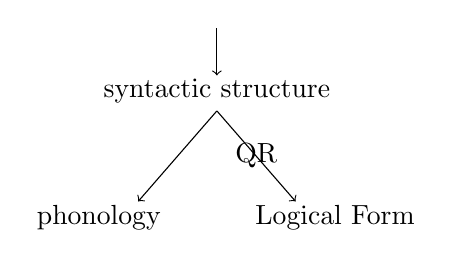
\begin{tikzpicture}
%\draw (0,1) node {deep structure};
\draw (0,0) node {syntactic structure};
\draw (-1.5,-1.6) node {phonology};
\draw (1.5,-1.6) node {Logical Form};
\draw (0,0.8) edge[->] (0,0.2);
\draw (0,-0.25) edge[->] (-1,-1.4); 
\path (0,-0.25) edge[->] node {{QR}} (1,-1.4);
\end{tikzpicture}
\end{center}
\end{frame}
\end{comment} 

\begin{frame}{Solution 2: Extracting quantifiers}

\begin{itemize}
\item {\bf Quantifier raising}
\item The same effect can be achieved by a semantic rule, e.g. 
{Montague's {\bf Quantifying in} rule}.
Here is our version of it:
\begin{align*}
\textbf{VP} &\to \textbf{TV\ \ NP}\\
\sem{\textbf{VP}} &= \lambda y.(\sem{\textbf{NP}}\ \lambda x.((\sem{\textbf{TV}}\ x)\ y))
\end{align*}
\end{itemize}
\end{frame}


\section{Interpreting our grammar and implementation}

\begin{frame}{}

\begin{center}
{\Large Interpreting our grammar and implementation}
\end{center}
\end{frame}

\begin{frame}[fragile]{The picture}

\begin{center}
\only<1>{string $\longrightarrow$ tree structure $\longrightarrow$ meaning representation}%
\only<2>{string $\longrightarrow$ \alert{tree structure $\longrightarrow$ meaning representation}}
\end{center}\pause

We will now consider tree structures and how to map them to expressions of typed lambda calculus.

\vspace{.4cm}

\begin{code}
module Day3 where

import Day2 hiding (Tree(..))
\end{code}
\end{frame}

\begin{frame}{Our grammar}

\begin{align*}
  \textbf{S} & ::= \textbf{NP}\ \ \textbf{VP} \\
\textbf{NP} & ::= \textbf{NAME} \mid \textbf{DET}\ \ \textbf{N} \mid \textbf{DET\ \ RN} \\
\textbf{ADJ} & ::= \text{\em happy} \mid \text{\em drunken} \mid \text{\em evil}  \\
\textbf{NAME} & ::= \text{\em Atreyu} \mid \text{\em Dorothy} \mid \text{\em Goldilocks} \mid \text{\em Snow White} \\
\textbf{N} & ::= \text{\em boy} \mid \text{\em princess} \mid \text{\em dwarf} \mid \text{\em wizard}  \mid \textbf{ADJ} \ \ \textbf{N} \\
\textbf{RN} & ::= \textbf{N\ \ REL\ \ VP} \mid \textbf{N\ \ REL\ \ NP\ \ TV} \\
\textbf{REL} & ::= \text{\em that} \\
\textbf{DET} & ::= \text{\em some} \mid \text{\em every} \mid \text{\em no} \\
\textbf{VP} & ::= \textbf{IV} \mid \textbf{TV}\ \ \textbf{NP} \mid \textbf{DV\ \ NP\ \ NP} \\
\textbf{IV} & ::= \text{\em cheered} \mid \text{\em laughed} \mid \text{\em shuddered} \\
\textbf{TV} & ::= \text{\em admired} \mid \text{\em helped} \mid \text{\em defeated} \mid \text{\em found} \\
\textbf{DV} & ::= \text{\em gave} \\
\end{align*}
\end{frame}

\begin{frame}{Tree structures}

A {\bf parse tree} for a string generated by a grammar $G$ is a tree where:
\begin{itemize}
\item The root is the start symbol for $G$.
\item The interior nodes are nonterminals of $G$ and 
the children of a node $N$ correspond to the symbols on the right hand side of some production rule for $T$ in $G$. 
\item The leaf nodes are terminal symbols of $G$.
\end{itemize}

Every string generated by a grammar has a corresponding parse tree that illustrates a derivation for that string.
\end{frame}

\begin{frame}{Example}
 
{\em Every dwarf defeated some giant.} \\[.4cm] 
%{\tt\small S (NP Einige Ritter) (VP Verachten (NP Alle Schurken))}

{\small
\Tree [.{\bf S} [.{\bf NP} [.{\bf DET} {\em every} ] [.{\bf N} {\em dwarf} ] ] 
                [.{\bf VP} [.{\bf TV} {\em defeated} ] [.{\bf NP} [.{\bf DET} {\em some} ] [.{\bf N} {\em giant} ] ] ] ]
}
\end{frame}


\begin{frame}[fragile]{Parse trees}

A parse tree is either a leaf with information, or a branch with information 
dominating a list of trees.

\begin{code}
data Tree a b = Leaf a | Branch b [Tree a b]   deriving Show
\end{code}\pause

{\bf Example:}

\begin{code}
tree :: Tree String String
tree = Branch "S" [Branch "NP" [Branch "DET" [Leaf "every"], 
                                Branch "N"   [Leaf "dwarf"]], 
                   Branch "VP" [Branch "TV"  
                                           [Leaf "defeated"], 
                                Branch "NP" 
                                 [Branch "DET" [Leaf "some"],
                                  Branch "N"   [Leaf "giant"]]]]
\end{code}
\end{frame}

\begin{frame}[fragile]{Example}

{\footnotesize
\begin{verbatim}
tree :: Tree String String
tree = Branch "S" [Branch "NP" [Branch "DET" [Leaf "every"], 
                                Branch "N"   [Leaf "dwarf"]], 
                   Branch "VP" [Branch "TV"  [Leaf "defeated"], 
                                Branch "NP" [Branch "DET" [Leaf "some"],
                                             Branch "N"   [Leaf "giant"]]]]
\end{verbatim}
}
{%\small
\Tree [.{\tt S} [.{\tt NP} [.{\tt DET} {\tt every} ] [.{\tt N} {\tt dwarf} ] ] 
                [.{\tt VP} [.{\tt TV} {\tt defeated} ] [.{\tt NP} [.{\tt DET} {\tt some} ] [.{\tt N} {\tt giant} ] ] ] ]
}
\end{frame}


\begin{frame}{Implementation}

We define a mapping from parse trees to lambda expressions by recursion over 
the structure of a parse tree. For a sentence tree it will return the analogue 
of the predicate logical formula representing the meaning of this sentence. 

\vspace{.4cm}

{\bf General type:} {\tt Tree String String -> }$\text{\em map}(\tau)$, where
\begin{itemize}
\item $\text{\em map}(\tau_1\to\tau_2)=\text{\em map}(\tau_1)\text{\tt\ ->\ }\text{\em map}(\tau_2)$
\item $\text{\em map}(e)=\text{\tt Term}$
\item $\text{\em map}(t)=\text{\tt Formula}$
\end{itemize}
\end{frame}

\begin{frame}[fragile]{Interpretation and implementation}

\begin{align*}
&\quad \sem{\textbf{S}} :: t \\
\textbf{S} \to \textbf{NP\ \ VP} &\quad \sem{\textbf{S}} = (\sem{\textbf{NP}}\ \ \sem{\textbf{VP}}) \\
\end{align*}

\begin{code}
transS :: Tree String String -> Formula
transS (Branch "S" [np,vp]) = (transNP np) (transVP vp)
\end{code}
\end{frame}

\begin{frame}[fragile]{Interpretation and implementation}

\begin{align*}
&\quad \sem{\textbf{NP}} :: (e\to t)\to t \\
\textbf{NP} \to \textbf{NAME} &\quad \sem{\textbf{NP}} = \sem{\textbf{NAME}} \\
\textbf{NP} \to \textbf{DET}\ \ \textbf{N} &\quad \sem{\textbf{NP}} = (\sem{\textbf{DET}}\ \ \sem{\textbf{N}}) \\
\textbf{NP} \to \textbf{DET}\ \ \textbf{RN} &\quad \sem{\textbf{NP}} = (\sem{\textbf{DET}}\ \ \sem{\textbf{RN}})
\end{align*}

\begin{code}
transNP :: Tree String String -> (Term -> Formula) -> Formula 
transNP (Branch "NP" [name])   = transNAME name 
transNP (Branch "NP" [det,n@(Branch "N" ts)])   = 
                                 (transDET det) (transN n)
transNP (Branch "NP" [det,rn@(Branch "RN" ts)]) = 
                                 (transDET det) (transRN rn)
\end{code}
\end{frame}

\begin{frame}[fragile]{Interpretation and implementation}

\begin{align*}
&\quad \sem{\textbf{NAME}} :: (e\to t)\to t \\
\textbf{NAME} \to \text{\em Atreyu} &\quad \sem{\textbf{NAME}} = \lambda P.(P\ a) \\
\textbf{NAME} \to \text{\em Goldilocks} &\quad \sem{\textbf{NAME}} = \lambda P.(P\ b) \\
\textbf{NAME} \to \text{\em Dorothy} &\quad \sem{\textbf{NAME}} = \lambda P.(P\ d) \\
\end{align*}
\begin{code}
transNAME :: Tree String String -> (Term -> Formula) 
                                -> Formula 
transNAME (Branch "NAME" [Leaf "Atreyu"]) = 
                                        \ p -> p (Const "a") 
transNAME (Branch "NAME" [Leaf "Goldilocks"]) = 
                                        \ p -> p (Const "b") 
transNAME (Branch "NAME" [Leaf "Dorothy"]) = 
                                        \ p -> p (Const "d")
\end{code}
\end{frame}


\begin{frame}[fragile]{Interpretation and implementation}

\begin{align*}
&\quad \sem{\textbf{N}} :: e\to t \\
\textbf{N} \to \text{\em wizard} &\quad \sem{\textbf{N}} = \lambda x.(\text{\em wizard}\ x) \\
& \ldots \\
%\textbf{N} \to \text{\em princess} &\quad \sem{\textbf{N}} = \lambda x.(\text{\em princess}\ x) \\
%\textbf{N} \to \text{\em dwarf} &\quad \sem{\textbf{N}} = \lambda x.(\text{\em dwarf}\ x) \\ 
%\textbf{N} \to \text{\em wizard} &\quad \sem{\textbf{N}} = \lambda x.(\text{\em wizard}\ x) \\
\textbf{N} \to \textbf{ADJ\ \ N} &\quad \sem{\textbf{N}} = \lambda x.((\sem{\textbf{ADJ}}\ x)\land (\sem{\textbf{N}}\ x))
\end{align*}
\begin{code}
transN :: Tree String String -> Term -> Formula
transN (Branch "N" [Leaf "wizard"]) = 
                                \ x -> (Atom "wizard" [x])
transN (Branch "N" [Leaf "giant"]) = 
                                \ x -> (Atom "giant" [x])
transN (Branch "N" [Leaf "princess"]) = 
                                \ x -> (Atom "princess" [x])
transN (Branch "N" [Leaf "dwarf"]) = 
                                \ x -> (Atom "dwarf" [x])
transN (Branch "N" [adj,n]) = 
                     \ x -> Conj [transADJ adj x,transN n x]
\end{code}
\end{frame}


\begin{frame}[fragile]{Interpretation and implementation}

\begin{align*}
&\quad \sem{\textbf{ADJ}} :: e\to t \\
\textbf{ADJ} \to \text{\em happy} &\quad \sem{\textbf{ADJ}} = \lambda x.(\text{\em happy}\ x) \\
& \ldots 
%\textbf{ADJ} \to \text{\em drunken} &\quad \sem{\textbf{ADJ}} = \lambda x.(\text{\em drunken}\ x) \\
%\textbf{ADJ} \to \text{\em evil} &\quad \sem{\textbf{ADJ}} = \lambda x.(\text{\em evil}\ x) 
\end{align*}
\begin{code}
transADJ :: Tree String String -> Term -> Formula
transADJ (Branch "ADJ" [Leaf "happy"]) = 
                                  \ x -> Atom "happy" [x]
transADJ (Branch "ADJ" [Leaf "drunken"]) = 
                                  \ x -> Atom "drunken" [x]
transADJ (Branch "ADJ" [Leaf "evil"])  = 
                                  \ x -> Atom "evil" [x]
\end{code}
\end{frame}


\begin{frame}[fragile]{Interpretation and implementation}

\begin{align*}
&\quad \sem{\textbf{RN}} :: e\to t \\
\textbf{RN} \to \textbf{N\ REL\ VP} &\quad \sem{\textbf{RN}} = \lambda x.(\sem{\textbf{N}}\ x)\land (\sem{\textbf{VP}}\ x) \\
\textbf{RN} \to \textbf{N\ REL\ NP TV} &\quad \sem{\textbf{RN}} = \lambda x.(\sem{\textbf{N}}\ x)\land (\sem{\textbf{NP}}\ \lambda y.((\sem{\textbf{TV}}\ y)\ x)) 
\end{align*}
\begin{code}
transRN :: Tree String String -> Term -> Formula
transRN (Branch "RN" [n,rel,vp])    = 
              \ x -> Conj [(transN n x),(transVP vp x)]
transRN (Branch "RN" [n,rel,np,tv]) = 
              \ x -> Conj [(transN n x),(transNP np (\ y -> (transTV tv y x)))]
\end{code}
\end{frame}

\begin{frame}[fragile]{Interpretation and implementation}

\begin{align*}
&\quad \sem{\textbf{VP}} :: e\to t \\
\textbf{VP} \to \textbf{IV} &\quad \sem{\textbf{VP}} = \sem{\textbf{IV}} \\ 
\textbf{VP} \to \textbf{TV\ \ NP} &\quad \sem{\textbf{VP}} = \lambda y.(\sem{\textbf{NP}}\ \lambda x.((\sem{\textbf{TV}}\ x)\ y))\\
\textbf{VP} \to \textbf{DV\ \ NP\ \ NP} &\quad \sem{\textbf{VP}} = \lambda z.(\sem{\textbf{NP}}\ \lambda y.(\sem{\textbf{NP}}\ \lambda x.(((\sem{\textbf{TV}}\ x)\ y)\ z)))
\end{align*}
\begin{code}
transVP :: Tree String String -> Term -> Formula
transVP (Branch "VP" [iv]) = transIV iv 
transVP (Branch "VP" [tv,np]) = 
  \ y -> (transNP np)  (\ x -> (transTV tv) x y)
transVP (Branch "VP" [dv,np1,np2]) = 
  \ z -> (transNP np1) (\ y -> (transNP np2) 
                                (\ x -> (transDV dv) x y z))
\end{code}
\end{frame}

\begin{frame}[fragile]{Interpretation and implementation}

\begin{align*}
&\quad \sem{\textbf{IV}} :: e\to t \\
\textbf{IV} \to \text{\em cheered} &\quad \sem{\textbf{IV}} = \lambda x.(\text{\em cheered}\ x) \\
 & \ldots \\
%\textbf{IV} \to \text{\em laughed} &\quad \sem{\textbf{IV}} = \lambda x.(\text{\em laugh}\ x) \\
%\textbf{IV} \to \text{\em shuddered} &\quad \sem{\textbf{IV}} = \lambda x.(\text{\em shudder}\ x)  
\end{align*}
\begin{code}
transIV :: Tree String String -> Term -> Formula 
transIV (Branch "IV" [Leaf "cheered"]) = 
                                   \ x -> Atom "cheer" [x]
transIV (Branch "IV" [Leaf "laughed"]) = 
                                   \ x -> Atom "laugh" [x] 
transIV (Branch "IV" [Leaf "shuddered"]) = 
                                   \ x -> Atom "shudder" [x]  
\end{code}
\end{frame}

\begin{frame}[fragile]{Interpretation and implementation}

\begin{align*}
&\quad \sem{\textbf{TV}} :: e\to (e\to t) \\ 
\textbf{TV} \to \text{\em admired} &\quad \sem{\textbf{TV}} = \lambda x\lambda y.((\text{\em admire}\ x)\ y) \\
& \ldots \\
%\textbf{TV} \to \text{\em helped} &\quad \sem{\textbf{TV}} = \lambda x\lambda y.((\text{\em help}\ x)\ y) \\
%\textbf{TV} \to \text{\em defeated} &\quad \sem{\textbf{TV}} = \lambda x\lambda y.((\text{\em defeat}\ x)\ y) \\
%\textbf{TV} \to \text{\em found} &\quad \sem{\textbf{TV}} = \lambda x\lambda y.((\text{\em find}\ x)\ y)
\end{align*}
\begin{code}
transTV :: Tree String String -> Term -> Term -> Formula 
transTV (Branch "TV" [Leaf "admired"])  = 
                           \ x y -> Atom "admire" [y,x] 
transTV (Branch "TV" [Leaf "helped"])   = 
                           \ x y -> Atom "help"   [y,x] 
transTV (Branch "TV" [Leaf "defeated"]) = 
                           \ x y -> Atom "defeat" [y,x] 
transTV (Branch "TV" [Leaf "found"])    = 
                           \ x y -> Atom "find"   [y,x] 
\end{code}
\end{frame}

\begin{frame}[fragile]{Interpretation and implementation}

\begin{align*}
&\quad \sem{\textbf{DV}} :: e\to (e\to (e\to t)) \\
\textbf{DV} \to \text{\em gave} &\quad \sem{\textbf{TV}} = \lambda x\lambda y\lambda y.(((\text{\em give}\ x)\ y)\ z) \\
\end{align*}
\begin{code}
transDV :: Tree String String -> Term -> Term -> Term 
                                           -> Formula 
transDV (Branch "DV" [Leaf "gave"]) = 
                  \ x y z -> Atom "give" [z,y,x]
\end{code}
\end{frame}


\begin{frame}[fragile]{Interpretation and implementation}

\vspace{-.6cm}

\begin{align*}
&\quad \sem{\textbf{DET}}::(e\to t)\to (e\to t)\to t \\
\textbf{DET} \to \text{\em every} &\quad \sem{\textbf{DET}} = \lambda P\lambda Q.\forall x.((P\ x)\to(Q\ x)) \\ 
\textbf{DET} \to \text{\em some} &\quad \sem{\textbf{DET}} = \lambda P\lambda Q.\exists x.((P\ x)\to(Q\ x)) \\ 
\textbf{DET} \to \text{\em no} &\quad \sem{\textbf{DET}} = \lambda P\lambda Q.\lnot\exists x.((P\ x)\to(Q\ x)) 
\end{align*}
\begin{code}
transDET :: Tree String String -> (Term -> Formula) 
                               -> (Term -> Formula) 
                               -> Formula 
transDET (Branch "DET" [Leaf "every"]) p q = 
          Forall i (Impl (p (Var i)) (q (Var i))) 
                               where i = fresh [p,q]
transDET (Branch "DET" [Leaf "some"])  p q  = 
          Exists i (Conj [p (Var i),q (Var i)]) 
                               where i = fresh [p,q]
transDET (Branch "DET" [Leaf "no"])    p q = 
          Neg (Exists i (Conj [p (Var i),q (Var i)])) 
                               where i = fresh [p,q]
\end{code}
\end{frame}

\begin{frame}[fragile]{Fresh variables}

\ldots {\tt where i = fresh [p,q]}

\begin{code}
fresh :: [Term -> Formula] -> Int
fresh xs | vars == [] = 1
         | otherwise  = 1 + maximum vars
     where 
     vars = concat $ map (\ f -> getVars (f (Const "*"))) xs
\end{code}

Where {\tt getVars :: Formula -> [Int]} collects all variables occurring in a formula.
\end{frame}

\begin{frame}[fragile]{Collecting variables}

\begin{code}
getVars :: Formula -> [Int]
getVars (Atom _ ts)  = concat $ map getVar ts 
getVars (Neg  f)     = getVars f
getVars (Conj fs)    = concat $ map getVars fs
getVars (Disj fs)    = concat $ map getVars fs
getVars (Impl f1 f2) = getVars f1 ++ getVars f2
getVars (Forall n f) = n : getVars f
getVars (Exists n f) = n : getVars f

getVar :: Term -> [Int]
getVar (Const _) = []
getVar (Var   n) = [n]
\end{code}
\end{frame}

%\begin{frame}{Mapping parse trees to logical forms}
%
%Now we can map every parse tree to an expression that reduces to a first-order formula, 
%which can then be checked for truth with respect to a model.
%\end{frame}


\begin{frame}{Course overview}

\begin{itemize}
\item[] {\color{CWIgrey}{\bf Day 2:}\\ Meaning representations and (predicate) logic}
\item[] {\color{CWIgrey}{\bf Day 3:}\\ Lambda calculus and the composition of meanings}
\item {\bf Day 4:}\\ Extensionality and intensionality
\item {\bf Day 5:}\\ From strings to truth conditions and beyond
\end{itemize}
\end{frame}



\begin{comment}

\begin{frame}{Other challenges: inverse scope readings}

\begin{itemize}
\item {\tt Most Jedis survived all battles.}
% \begin{itemize} 
% \item Most Jedis $x$ are such that for all battles $y$ it holds that $x$ survived $y$.
% \item All battles $y$ are such that for most Jedis $x$ it holds that $x$ survived $y$.
% \end{itemize}
\item {\tt Most people think $[$that some Jedi escaped from Alderaan$]$.}
\item {\tt Most people think $[$that every Jedi escaped from Alderaan$]$.}
\end{itemize}
\end{frame}


\begin{frame}{Two kinds of approaches}

Either the \alert{syntactic structure} of the sentences is different... 
\begin{itemize}
\item covert movement of quantifiers (May's {\em Quantifier Raising})
\end{itemize}
...or the \alert{semantics} has to be adjusted.
\begin{itemize}
\item Montague's {\em Quantifying In} rule
\item Cooper stores, underspecified semantic representations
\item choice functions
\end{itemize}
\end{frame}


\end{comment}


\end{document}